\documentclass[8pt,sans,mathserif,aspectratio=43]{beamer}

\usepackage{ucs}
\usepackage[T1]{fontenc}
% \usepackage[utf8x]{inputenc}
\usepackage{CJKutf8}            % Japanese
\usepackage[english,greek]{babel}

\usepackage{kerkis}
% \usepackage{eulervm}
% \usepackage{courier}
% \usepackage{palatino}
% \usepackage{kmath}

\usepackage{time}
\usepackage{graphicx}
\usepackage{color}
\usepackage{amssymb,amsmath}
\usepackage{isomath}
\hypersetup{unicode}

% Beamer setup

\usetheme{default}
\useoutertheme{infolines-center}
\usecolortheme{whale}

\definecolor{blendedblue}{rgb}{0.037,0.366,0.551}

\setbeamercolor{structure}{fg=blendedblue}
\setbeamercolor{titlelike}{parent=structure}
\setbeamercolor{frametitle}{fg=black}
\setbeamercolor{title}{fg=black}
\setbeamercolor{item}{fg=black}

% \setbeamercovered{transparent}
\setbeamercovered{invisible}

\setbeamertemplate{footline}{}
\setbeamertemplate{navigation symbols}{}

\defbeamertemplate*{title page}{customized}[1][]
{\centering{
    \vfill
    \usebeamerfont{title}\inserttitle\par
    \vfill
    \usebeamerfont{subtitle}\usebeamercolor[fg]{subtitle}\insertsubtitle\par
    \vfill
    \usebeamercolor[fg]{titlegraphic}\inserttitlegraphic
    \vfill
    \usebeamerfont{author}\insertauthor\par
    \vfill
    \usebeamerfont{institute}\insertinstitute\par
    \vfill
    \usebeamerfont{date}\insertdate\par
    \vfill
  }
}

% New commands-environments

\newcommand{\eng}[1]{\selectlanguage{english}#1\selectlanguage{greek}}
\newcommand{\gre}[1]{\selectlanguage{greek}#1\selectlanguage{english}}
\newcommand{\ttt}[1]{\selectlanguage{english}\texttt{#1}\selectlanguage{greek}}

\newcommand {\framedgraphic}[3]{
  \begin{frame}{#1}
    \begin{center}
      \includegraphics[width=\textwidth, keepaspectratio]
      {#2}\let\thefootnote\relax\footnote{#3}
    \end{center}
  \end{frame}
}

\newcommand{\spacer}[0]{
  \vspace{5pt}}

\newenvironment{Japanese}{%
  \CJKfamily{goth}%
  \CJKtilde
  \CJKnospace
}{}

\newcommand{\jap}[1]{%
  \begin{CJK}{UTF8}{}%
    \begin{Japanese}%
      \normalsize{#1}%
    \end{Japanese}%
  \end{CJK}%
}

\begin{document}

\title{Προσομοίωση Πρόσπτωσης \eng{Tsunami} \jap{(津波)} σε Ακτογραμμή}
\titlegraphic{\includegraphics[width=0.8\textwidth]{figures/paraview.png}}
\author{Αριστοτέλης Σπαθής-Παπαδιώτης} \institute{Τμήμα ΗΜ\&ΤΥ, Πανεπιστήμιο Πατρών}
\date{24 Φεβρουαρίου 2016}

%%%%%%%%%%%%%%%%%%%%%%%%%%%%%%%%%%%%%%%%%%%%%%%%%%%%%%%%%%%%%%%%%%%%%%%%%%%%%%%% 

\begin{frame}
  \titlepage
\end{frame}

%%%%%%%%%%%%%%%%%%%%%%%%%%%%%%%%%%%%%%%%%%%%%%%%%%%%%%%%%%%%%%%%%%%%%%%%%%%%%%%% 

\section{Εισαγωγή}

\begin{frame}
  \begin{columns}[T]
    \begin{column}{.58\textwidth}
      \begin{block}{}
        \begin{center}
          {\LARGEΣτόχος}

          \vspace{20pt}

          Η ανάπτυξη ενός ακριβούς, παραμετρικού προσομοιωτή δυναμικής ασυμπίεστων ρευστών
          και καταγραφής της αλληλεπίδρασής τους με το περιβάλλον
        \end{center}
      \end{block}
    \end{column}
  \end{columns}
\end{frame}

%%%%%%%%%%%%%%%%%%%%%%%%%%%%%%%%%%%%%%%%%%%%%%%%%%%%%%%%%%%%%%%%%%%%%%%%%%%%%%%% 

\framedgraphic{} {figures/tsunami-hit.jpg} {Από \ttt{www.theatlantic.com}}

%%%%%%%%%%%%%%%%%%%%%%%%%%%%%%%%%%%%%%%%%%%%%%%%%%%%%%%%%%%%%%%%%%%%%%%%%%%%%%%% 

\begin{frame}{Η γένεση ενός \eng{tsunami}}
  \includegraphics[width=0.5\textwidth]{figures/tsunami-gen-0.pdf}
  \includegraphics[width=0.5\textwidth]{figures/tsunami-gen-1.pdf}\\
  \includegraphics[width=0.5\textwidth]{figures/tsunami-gen-2.pdf}
  \includegraphics[width=0.5\textwidth]{figures/tsunami-gen-3.pdf}
  \let\thefootnote\relax\footnote{Από \eng{U.S. Geological Survey, Circular 1187}}
\end{frame}

%%%%%%%%%%%%%%%%%%%%%%%%%%%%%%%%%%%%%%%%%%%%%%%%%%%%%%%%%%%%%%%%%%%%%%%%%%%%%%%% 

\section{Μεθοδολογία Προσομοίωσης}
\subsection{Ρευστοδυναμική}

\begin{frame}
  \begin{columns}[T]

    \begin{column}{.5\textwidth}
      \begin{block}{}
        Εξίσωση \eng{Navier-Stokes}:
        $$
        \rho
        \left( \frac{\partial \vec{v}}{\partial t}
          + \vec{v} \cdot \nabla \vec{v}
        \right)
        =
        - \nabla p
        + \nabla \cdot \mathbb{T}
        + \vec{f},
        $$
        όπου
        \begin{itemize}
        \item $\rho$ η πυκνότητα
        \item $\vec{v}$ η ταχύτητα
        \item $p$ η πίεση
        \item $\mathbb{T}$ o όρος παραμόρφωσης του τανυστή τάσης
        \item $\vec{f}$ η δύναμη ανά μονάδα όγκου
        \end{itemize}
        Η εξίσωση είναι ισχυρά μη γραμμική, ενώ υπάρχουν πολλές μέθοδοι για τη
        λύση της. \spacer

        \pause
        Δύο κύριες κατηγορίες μεθόδων:
        \begin{itemize}
        \item Αριθμητικές -- χρησιμοποιούν δίκτυο (\eng{mesh-based})
        \item Σωματιδιακές -- δεν χρησιμοποιούν δίκτυο (\eng{meshfree})
          \begin{itemize}
          \item \eng{Lattice Boltzmann method}
          \item \eng{Smoothed-particle hydrodynamics}
          \end{itemize}
        \end{itemize}
      \end{block}
    \end{column}

    \begin{column}{.4\textwidth}
      \begin{block}{}
        \visible<2->{\includegraphics[width=0.85\textwidth]{figures/fem.png}}
      \end{block}
    \end{column}
  \end{columns}

  \onslide<1->\let\thefootnote\relax\footnote{Εικόνες από \ttt{en.wikipedia.org}}
\end{frame}

%%%%%%%%%%%%%%%%%%%%%%%%%%%%%%%%%%%%%%%%%%%%%%%%%%%%%%%%%%%%%%%%%%%%%%%%%%%%%%%% 

\subsection{\texorpdfstring{\eng{LBM}}{LBM}}

\begin{frame}{\eng{Lattice Boltzmann Method}}

  \begin{columns}[T]

    \begin{column}{.6\textwidth}
      \begin{block}{}
        Προέρχεται από τα \eng{Lattice Gas Cellular Automata (LGCA)}\spacer

        Χρησιμοποιεί τη διακριτοποιημένη στο χώρο και το χρόνο μορφή της
        εξίσωσης \eng{Boltzmann}:
        $$
        \frac{\partial f}{\partial t}
        + \vec{v} \cdot \nabla f
        + \vec{F} \cdot \nabla_{\vec{p}}\hspace{2pt} f
        = \Omega(f),
        $$
        όπου
        \begin{itemize}
        \item $f$ η κατανομή στο χώρο των φάσεων
        \item $\vec{v}$ η ταχύτητα
        \item $\vec{F}$ η εξωτερική δύναμη
        \item $\vec{p}$ η ορμή
        \item $\Omega(f)$ ο τελεστής σύγκρουσης
        \end{itemize}
        \spacer
        \pause

        Επαναληπτική εκτέλεση δύο βημάτων:
        \begin{itemize}
        \item \eng{Collision:}
          $f_i^t(\vec{x},t+\delta_t) = f_i(\vec{x},t)+\frac{1}{\tau_f}(f_i^{eq}-f_i)$
        \item \eng{Streaming:}
          $f_i(\vec{x}+\vec{v}\delta_t, t+\delta_t)=f_i^t(\vec{x},t+\delta_t),$
        \end{itemize}
        όπου $\tau_f$ η παράμετρος χαλάρωσης και $f_i^{eq}$ η κατανομή σε
        θερμοδυναμική ισορροπία για την προσέγγιση του τελεστή σύγκρουσης κατά
        \eng{BGK}.
      \end{block}
    \end{column}

    \begin{column}{.4\textwidth}
      \begin{block}{}
        \visible<2->{\includegraphics[width=.7\textwidth]{figures/lbm.png}}
      \end{block}
    \end{column}
  \end{columns}

  \onslide<1->\let\thefootnote\relax\footnote{Εικόνες από \ttt{science.uva.nl}
    και \ttt{scholarpedia.org}}
\end{frame}

%%%%%%%%%%%%%%%%%%%%%%%%%%%%%%%%%%%%%%%%%%%%%%%%%%%%%%%%%%%%%%%%%%%%%%%%%%%%%%%% 

\subsection{\texorpdfstring{\eng{SPH}}{SPH}}

\begin{frame}{Θεωρητική θεμελίωση}
  Ξεκινάμε από την ταυτότητα δειγματοληψίας
  \begin{equation*}
    f(\vec{r}) = \int_Vf(\vec{x}) \delta(\vec{r} - \vec{x}) d\vec{x},
  \end{equation*}
  \pause αντικαθιστώντας την $\delta(\vec{r})$ με έναν γενικότερο πυρήνα εξομάλυνσης
  $W(\vec{r}, h)$ τέτοιο ώστε
  \begin{equation*}
    \lim_{h\to0}W(\vec{r}, h) = \delta(\vec{r})\ \ \
    \text{και}\ \ \
    \int_VW(\vec{r}, h) d\vec{x} = 1
  \end{equation*}
  \pause λαμβάνουμε έναν προσεγγιστικό εκτιμητή για την $f$
  \begin{equation*}
    f(\vec{r}) \approx \int_V f(\vec{x}) W(\vec{r}-\vec{x}, h) d\vec{x}
  \end{equation*}
  \pause Αν διακριτοποιήσουμε το πεδίο $f$ ο εκτιμητής μετασχηματίζεται σε διακριτό
  άθροισμα
  \begin{equation*}
    f(\vec{r}) \approx \sum_i \frac{\rho_i d\vec{x}}{\rho_i} f(\vec{r}_i) W(\vec{r}-\vec{r}_i, h)
    = \sum_i \frac{m_i}{\rho_i} f(\vec{r}_i) W(\vec{r}-\vec{r}_i, h)
  \end{equation*}
  όπου κάθε σημείο $i$ συνεισφέρει ανάλογα με το λόγο της μάζας του $m_i$ προς την τοπική
  πυκνότητα $\rho_i$.
\end{frame}

%%%%%%%%%%%%%%%%%%%%%%%%%%%%%%%%%%%%%%%%%%%%%%%%%%%%%%%%%%%%%%%%%%%%%%%%%%%%%%%% 

\begin{frame}{Βάθμωση και απόκλιση}
  Ένα ελκυστικό χαρακτηριστικό της \eng{SPH} είναι η αποκλειστική εξάρτηση των
  διανυσματικών τελεστών από τους αντίστοιχους του πυρήνα εξομάλυνσης $W$
  \begin{equation*}
    \nabla A(\vec{r}) = \sum_i \frac{m_i}{\rho_i} A(\vec{r}_i) \nabla W(\vec{r} - \vec{r}_i, h)
  \end{equation*}
  \pause Για την εξασφάλιση συμμετρίας δυνάμεων όπως αυτών που δημιουργούνται από τη
  βάθμωση της πίεσης $P$, μπορούμε να εξάγουμε εναλλακτικούς εκτιμητές. Από την ταυτότητα
  του γινομένου
  \begin{equation*}
    \label{eq:grad-identity}
    \nabla \left( \frac{P}{\rho} \right) =
    \frac{\nabla P}{\rho}-
    \frac{P}{\rho^2} \nabla \rho
    \hspace{10pt} \Leftrightarrow \hspace{10pt}
    \nabla P = \rho \left[ \frac{P}{\rho^2} \nabla \rho + \nabla \left( \frac{P}{\rho}
      \right) \right]
  \end{equation*}
  \pause αντικαθιστώντας στο δεξί μέλος τις βαθμώσεις με τους εκτιμητές τους κατά
  \eng{SPH}
  \begin{align}
    \label{eq:grad-est}
    \nabla P & = \rho \left[ \frac{P}{\rho^2} \sum_i \frac{m_i}{\rho_i} \rho_i \nabla
               W(\vec{r}-\vec{r}_i, h)
               +
               \sum_i \frac{m_i}{\rho_i} \frac{P_i}{\rho_i} \nabla W(\vec{r}-\vec{r}_i, h)
               \right] \nonumber \\
             & = \rho \sum_i m_i \left(\frac{P}{\rho^2} + \frac{P_i}{\rho_i^2} \right)
               \nabla W(\vec{r}-\vec{r}_i, h) \nonumber
  \end{align}
  \pause
  Αντίστοιχα για τη λαπλασιανή του διανυσματικού πεδίου ταχύτητας $\vec{v}$
  \begin{equation*}
    \label{eq:lapl-est}
    \nabla^2\vec{v} = \sum_i \frac{m_i}{\rho_i} (\vec{v}_i - \vec{v}) \nabla^2
    W(\vec{r}-\vec{r}_i, h)
  \end{equation*}

\end{frame}

%%%%%%%%%%%%%%%%%%%%%%%%%%%%%%%%%%%%%%%%%%%%%%%%%%%%%%%%%%%%%%%%%%%%%%%%%%%%%%%% 

\begin{frame} {Καταστατική εξίσωση και πυρήνες εξομάλυνσης}
  Η καταστατική εξίσωση χρησιμοποιείται για τον υπολογισμό της πίεσης από την τοπική
  πυκνότητα.
  \begin{columns}
    \begin{column}{.2\textwidth}
      \begin{equation*}
        P = k(\rho - \rho_0)
      \end{equation*}
    \end{column}
    \begin{column}{.2\textwidth}
      \begin{equation*}
        P = B \left( \left( \frac{\rho}{\rho_0} \right)^\gamma - 1 \right)
      \end{equation*}
    \end{column}
  \end{columns}
  \pause \vspace{10pt} Συνήθης πρακτική να χρησιμοποιούνται διαφορετικοί πυρήνες
  εξομάλυνσης για κάθε μέγεθος
  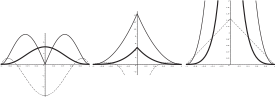
\includegraphics[width=\textwidth]{figures/smoothing-kernels.pdf}\\
  \hspace{38pt} Πυκνότητα \hspace{87pt} Πίεση \hspace{95pt} Ιξώδες

  \onslide<1->\let\thefootnote\relax\footnote{Εικόνα από \eng{M{\"u}ller et al., 2003}}
\end{frame}

%%%%%%%%%%%%%%%%%%%%%%%%%%%%%%%%%%%%%%%%%%%%%%%%%%%%%%%%%%%%%%%%%%%%%%%%%%%%%%%% 

\begin{frame}{Πλεονεκτήματα}
  \begin{itemize}
  \item Εγγενής διατήρηση πολλών μεγεθών στο σύστημα, όπως μάζα, ορμή και ενέργεια.\pause
  \item Ακριβής, ισότροπος και αμετάβλητος σε κάθε αδρανειακό σύστημα αναφοράς
    (\eng{Galilean invariant}) χειρισμός της καθαρής μεταφοράς (\eng{pure advection})\pause
  \item Δυνατότητα προσαρμογής της αναλυτικότητας (\eng{resolution}) και κατά συνέπεια του
    υπολογιστικού φόρτου δυναμικά συναρτήσει της θέσης, χρόνου ή άλλων παραγόντων.\pause
  \item Εύκολος χειρισμός ορίων και ειδικών αλληλεπιδράσεων σε εφαρμογές πολλαπλών φάσεων
    και συστατικών, μέσω των σωματιδιακών αλληλεπιδράσεων.
  \end{itemize}
  \includegraphics[width=\textwidth]{figures/boundary-particles.pdf}
  \onslide<1->\let\thefootnote\relax\footnote{Εικόνα από \eng{Akinci et al., 2012}}
\end{frame}

%%%%%%%%%%%%%%%%%%%%%%%%%%%%%%%%%%%%%%%%%%%%%%%%%%%%%%%%%%%%%%%%%%%%%%%%%%%%%%%% 

\section{Υλοποίηση}

\begin{frame}{Αρχιτεκτονική}
  \begin{center}
    \includegraphics[width=\textwidth, keepaspectratio]{figures/architecture.pdf}
  \end{center}
\end{frame}

%%%%%%%%%%%%%%%%%%%%%%%%%%%%%%%%%%%%%%%%%%%%%%%%%%%%%%%%%%%%%%%%%%%%%%%%%%%%%%%% 

\subsection{\texorpdfstring{\eng{Bullet}}{Bullet}}

\begin{frame}{\eng{Bullet}}
  \begin{columns}
    \begin{column}{.5\textwidth}
      \begin{itemize}
      \item Μηχανή προσομοίωσης μηχανικών αλληλεπιδράσεων
      \item Ευέλικτη αντικειμενοστραφής αρχιτεκτονική
      \item Μηχανική στερεών και μαλακών σωμάτων με διακριτή και συνεχή ανίχνευση συγκρούσεων.
      \item Υποστηρίζει διάφορα σχήματα συγκρούσεων όπως σφαίρα, ορθογώνιο παραλληλεπίπεδο,
        κύλινδρο, κώνο και τριγωνικά πλέγματα επιφάνειας
      \item Δυνατότητα εφαρμογής κίνησης, γεωμετρικών περιορισμών, δυνάμεων, ώσεων
      \item Λεπτομερής καταγραφή πολλαπλών πληροφοριών για κάθε αλληλεπίδραση
      \item \eng{Position Based Fluids}
      \end{itemize}
    \end{column}
    \begin{column}{.5\textwidth}
      \includegraphics[width=.8\textwidth, keepaspectratio]{figures/bullet-logo.png}
      \vspace{20pt}
      \includegraphics[width=.8\textwidth, keepaspectratio]{figures/bullet-wall.png}
    \end{column}
  \end{columns}
  \onslide<1->\let\thefootnote\relax\footnote{Εικόνες από \ttt{en.wikipedia.org}}
\end{frame}

%%%%%%%%%%%%%%%%%%%%%%%%%%%%%%%%%%%%%%%%%%%%%%%%%%%%%%%%%%%%%%%%%%%%%%%%%%%%%%%% 

\subsection{\texorpdfstring{Μηχανή \eng{SPH}}{SPH}}
\begin{frame}{\eng{LP grid}}
  Ειδική δομή για τη βελτιστοποίηση της αποθήκευσης και πρόσβασης στα σωματίδια.\\
  Ο χώρος της προσομοίωσης διαιρείται σε κανονικό πλέγμα κυβικών κελιών, μήκους ακμής
  $h$.\pause
  \begin{itemize}
  \item Συνεκτική αποθήκευση των σωματιδίων. Δεσμεύεται χώρος στη μνήμη ακριβώς ίσος με τον
    ελάχιστο δυνατό βάσει του μεγέθους της εσωτερικής αναπαράστασης των σωματιδίων.\pause
  \item Γρήγορη $Ο(1)$ πρόσβαση. Η ανάκτηση των σωματιδίων με βάση τη θέση τους γίνεται με
    λογική \eng{hash table} και είναι εγγυημένο οτι βρίσκονται όλα σε συνεχή περιοχή της
    μνήμης.\pause
  \item Ενημέρωση \eng{in-place}. Η ενημέρωση της δομής μετά από κάθε βήμα της προσομοίωσης
    δεν απαιτεί καμία επαναδεύσμευση (\eng{reallocation}) μνήμης και απαιτεί κατά κανόνα
    μικρό χρόνο.\pause
  \item Διατήρηση της τοπικότητας στην διάταξη αποθήκευσης. Τα σωματίδια κάθε κελιού είναι
    εγγυημένα αποθηκευμένα σε συνεχή περιοχή της μνήμης, ενώ σωματίδια γειτονικών κελιών
    βρίσκονται σε γειτονικές περιοχές της μνήμης, γεγονός που βελτιστοποιεί τη χρήση της
    κρυφής μνήμης σε υπολογισμούς αλληλεπιδράσεων εξαρτώμενων από την απόσταση στο
    χώρο.\pause
  \end{itemize}
  \includegraphics[width=\textwidth]{figures/lp-grid.pdf}

\end{frame}

%%%%%%%%%%%%%%%%%%%%%%%%%%%%%%%%%%%%%%%%%%%%%%%%%%%%%%%%%%%%%%%%%%%%%%%%%%%%%%%% 

\begin{frame}{Αρχικοποίηση}
  \begin{columns}
    \begin{column}{.7\textwidth}
      Ακτογραμμή:
      \begin{itemize}
      \item Εισαγωγή γεωμετρίας από κατάλληλο αρχείο περιγραφής
      \item Κλιμάκωση και μετακίνηση του μοντέλου στην αρχή των αξόνων
      \item Προσθήκη AABB και τυχόν επιπρόσθετων στοιχείων (λ.χ. κυματοθραύστης)
      \item Εξαγωγή πληροφορίας τελικών διαστάσεων χώρου προσομοίωσης
      \end{itemize}
      \pause
      Ρευστό:
      \begin{itemize}
      \item Εισαγωγή αρχικών συνθηκών ρευστού
      \item Διακριτοποίηση σε σωματίδια σε διάταξη \eng{HCP}
      \item Προσδιορισμός ακτίνας εξομάλυνσης $h$
      \item Προσαρμογή καταστατικής εξίσωσης
      \item Καταμέτρηση γειτονικών σωματιδίων
      \item Χρονικό βήμα (κριτήριο \eng{Courant-Friedrichs-Lewy}: $\delta t = C * \delta x/v$)
      \end{itemize}
      \pause
      \eng{LP grid}:
      \begin{itemize}
      \item Διαχωρισμός χώρου προσομοίωσης σε κυβικά κελιά ακμής $h$
      \item Δέσμευση μνήμης για την αποθήκευση των δεδομένων της προσομοίωσης
      \item Αρχική αποθήκευση σωματιδίων στη δομή
      \end{itemize}
    \end{column}
    \begin{column}{.3\textwidth}
      \onslide<2->
      \includegraphics[width=\textwidth]{figures/hcp.pdf}
      \vspace{10pt}
      \includegraphics[width=\textwidth]{figures/hcp-sphere.png}
    \end{column}
  \end{columns}
  \onslide<1->\let\thefootnote\relax\footnote{Εικόνες από \ttt{en.wikipedia.org} και
    \eng{Diehl et al.}, 2012, τροποποιημένες}
\end{frame}

%%%%%%%%%%%%%%%%%%%%%%%%%%%%%%%%%%%%%%%%%%%%%%%%%%%%%%%%%%%%%%%%%%%%%%%%%%%%%%%% 

\begin{frame}{Βήματα βρόχου προσομοίωσης}
  \begin{enumerate}
  \item Καθαρισμός δεδομένων των σωματιδίων που πρόκειται να επανυπολογιστούν \pause
  \item Ανιχνευση αλληλεπιδράσεων με παράλληλη σάρωση όλου του πλέγματος \pause
  \item Υπολογισμός πυκνότητας στις θέσεις των σωματιδίων μέσω προοδευτικής άθροισης των
    αμοιβαίων συνεισφορών των αλληλεπιδρώντων ζευγών \pause
  \item Υπολογισμός πίεσης μέσω της καταστατικής εξίσωσης του ρευστού, συναρτήσει της
    πυκνότητας \pause
  \item Υπολογισμός και εφαρμογή των ώσεων που υπολογίζονται ως το γινόμενο των δυνάμεων
    πίεσης/ιξώδους και του χρονικού βήματος, αντισυμμετρικών για κάθε ζεύγος
    αλληλεπίδρασης \pause
  \item Καταγραφή/αποθήκευση των ώσεων (\eng{impulses}) του ρευστού προς την ακτογραμμή
    \pause
  \item Ενημέρωση του πλέγματος αποθήκευσης των σωματιδίων \pause
  \item Υπολογισμός χρωματικού πεδίου και συνεισφοράς στο αθροιστικό πεδίο ώσεων \pause
  \end{enumerate}
  \begin{center}
    \includegraphics[width=0.75\textwidth]{figures/performance.pdf}
  \end{center}
\end{frame}

%%%%%%%%%%%%%%%%%%%%%%%%%%%%%%%%%%%%%%%%%%%%%%%%%%%%%%%%%%%%%%%%%%%%%%%%%%%%%%%%

\section{Αποτελέσματα}
\subsection{Ρευστό}

\begin{frame}{Διαδραστική οπτικοποίηση}
  \includegraphics[width=\textwidth]{figures/paraview.png}
\end{frame}

%%%%%%%%%%%%%%%%%%%%%%%%%%%%%%%%%%%%%%%%%%%%%%%%%%%%%%%%%%%%%%%%%%%%%%%%%%%%%%%% 

\begin{frame}{Πίεση}
  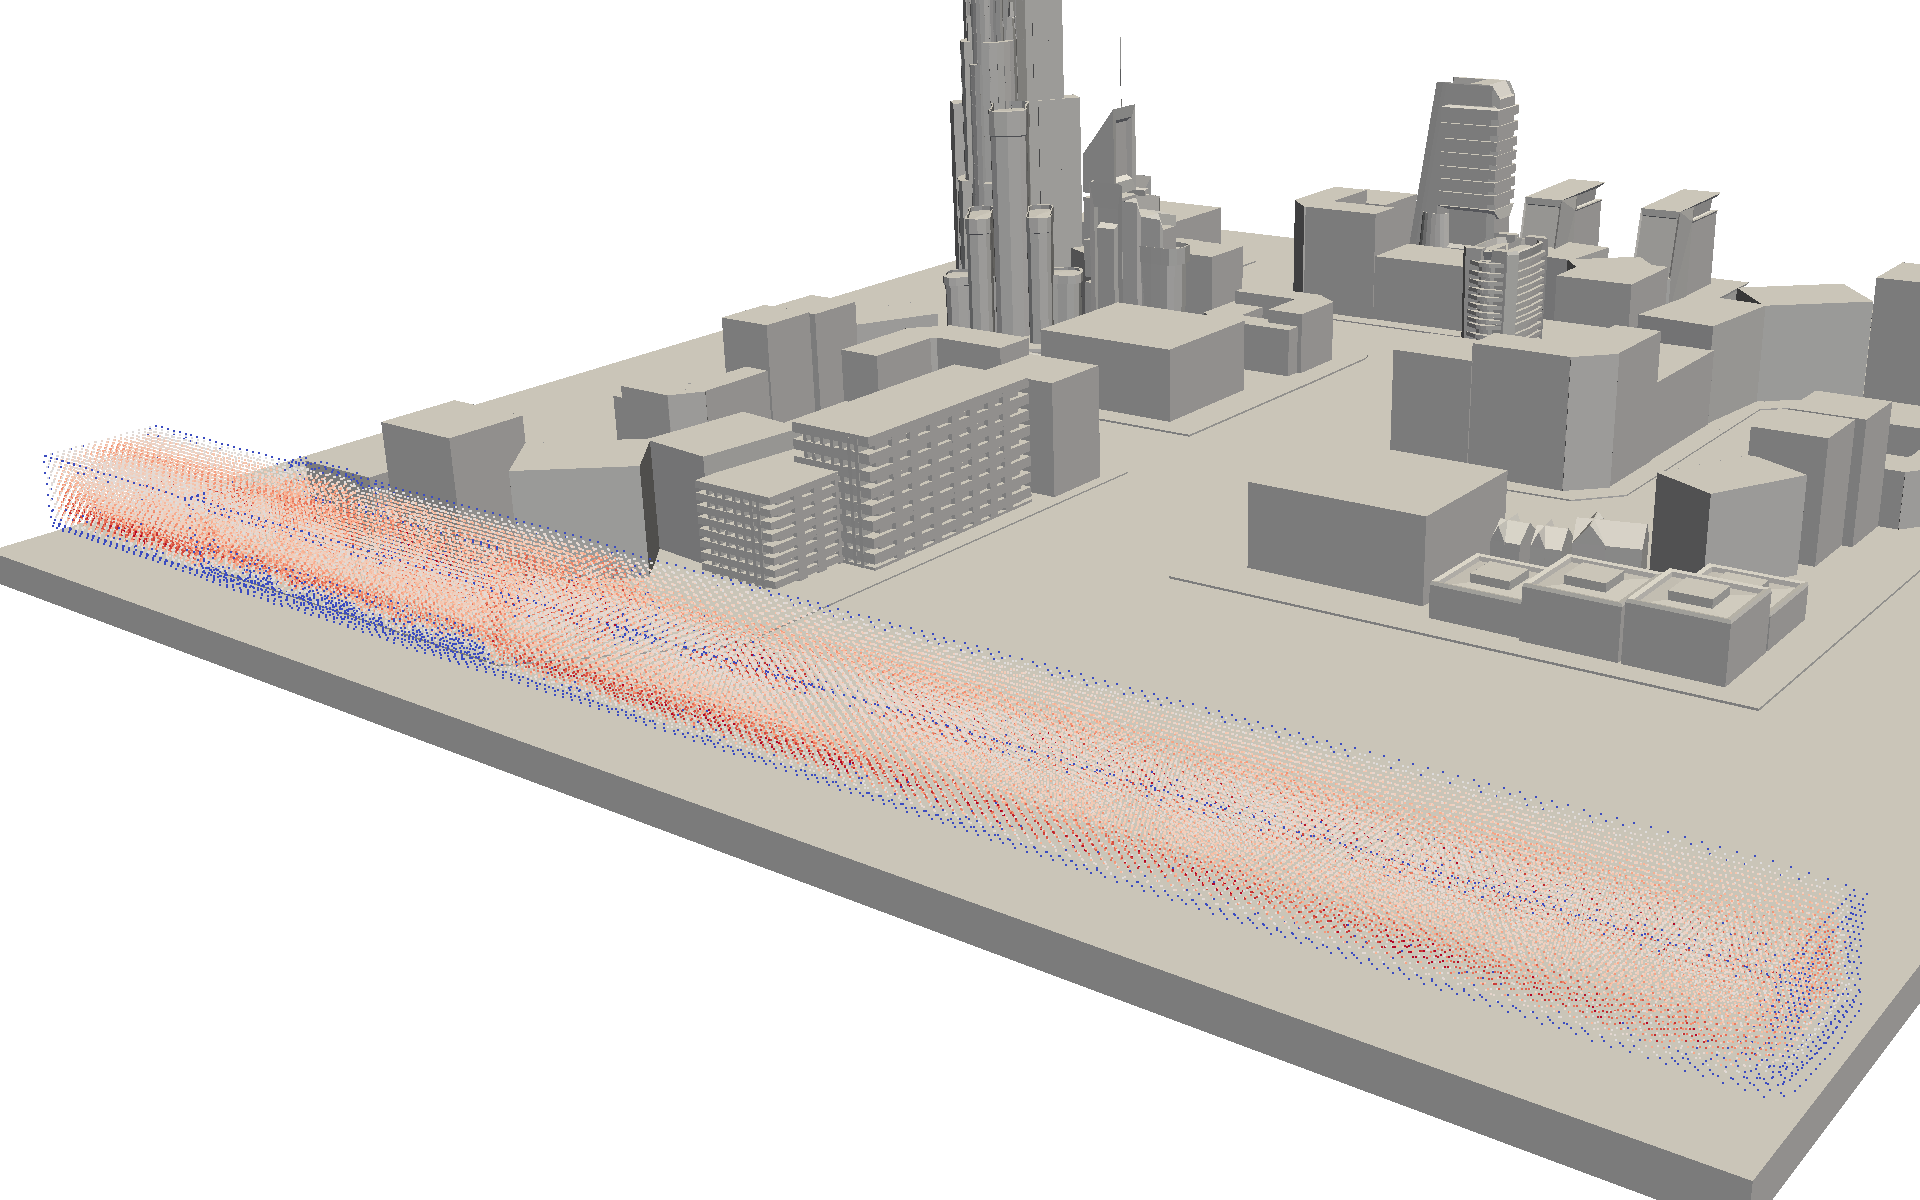
\includegraphics[width=.5\textwidth]{figures/press-0.png}
  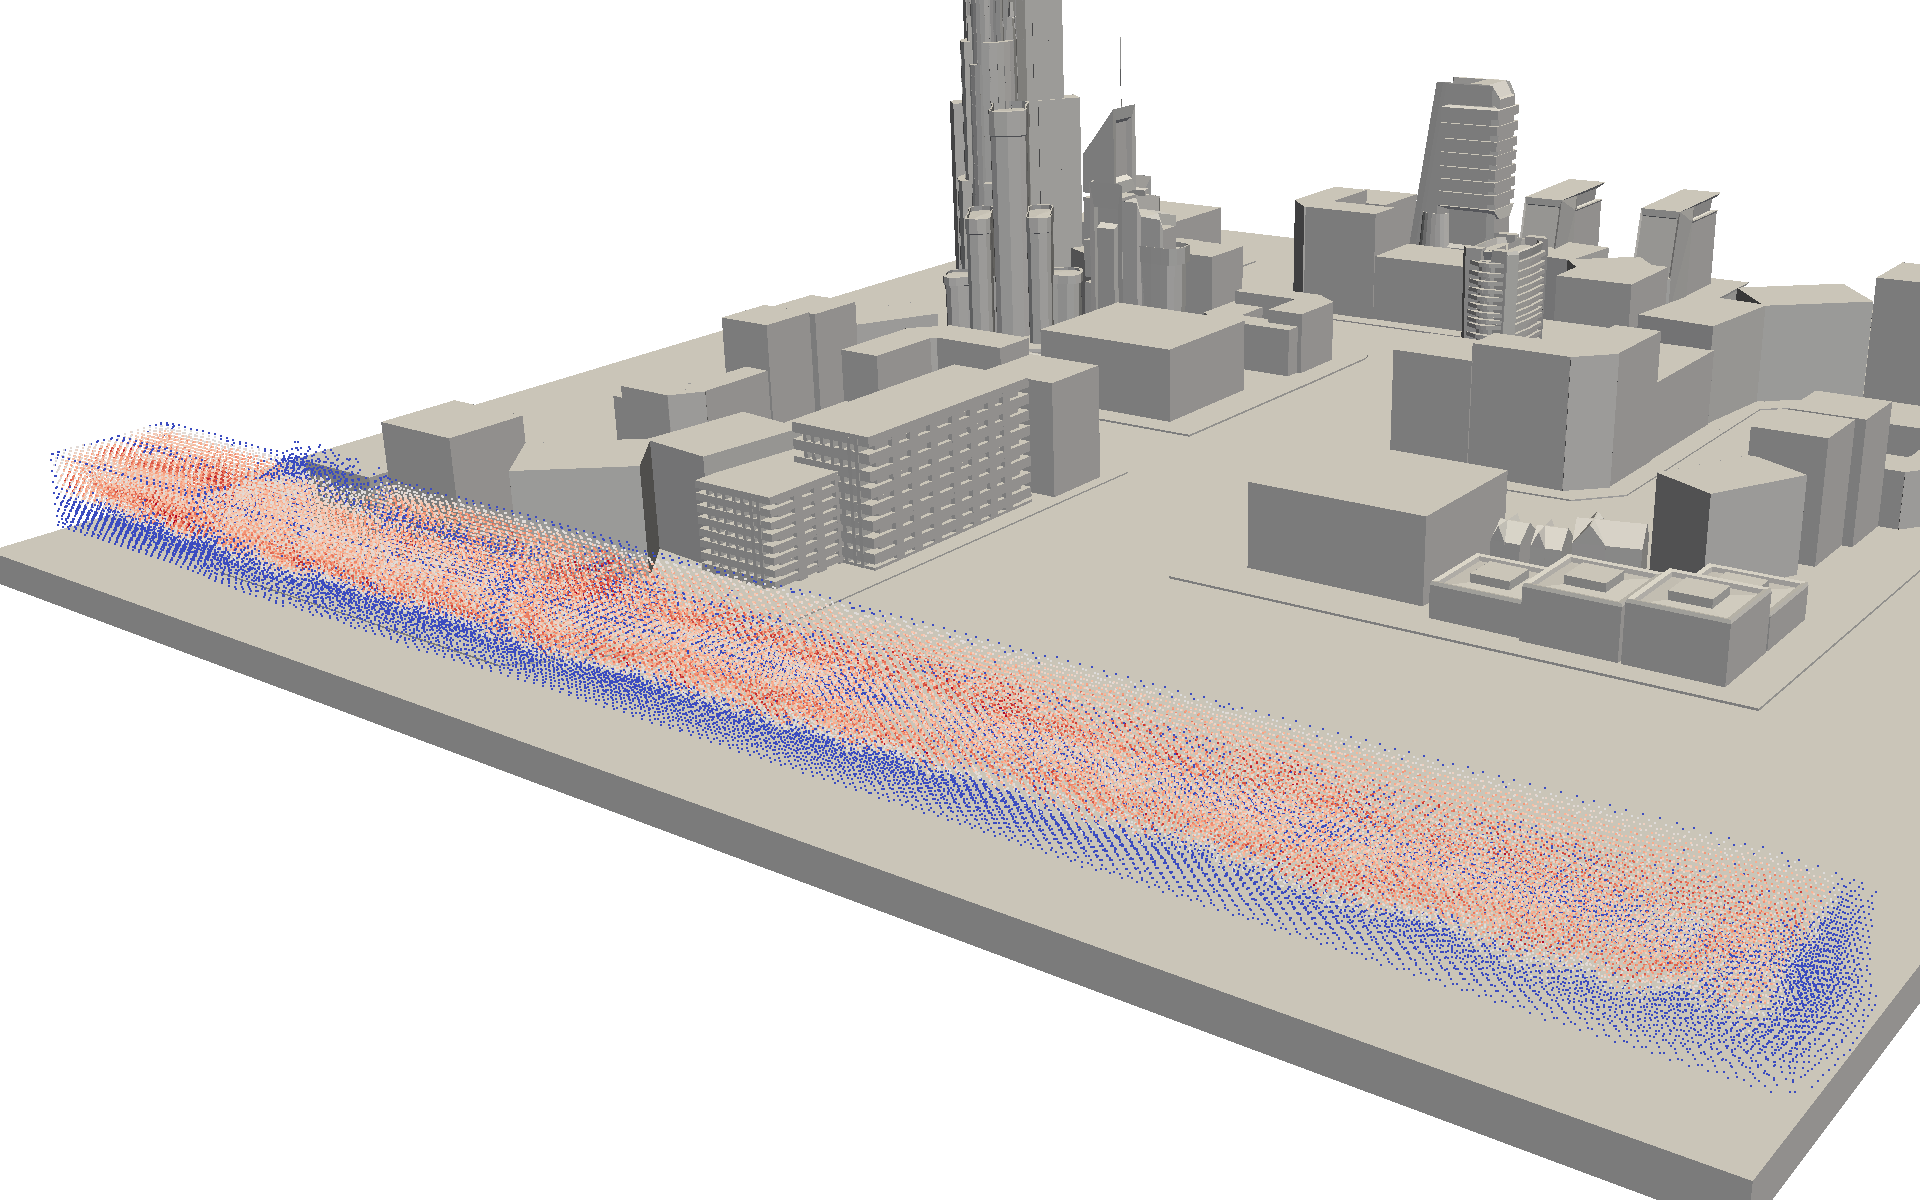
\includegraphics[width=.5\textwidth]{figures/press-1.png}\\
  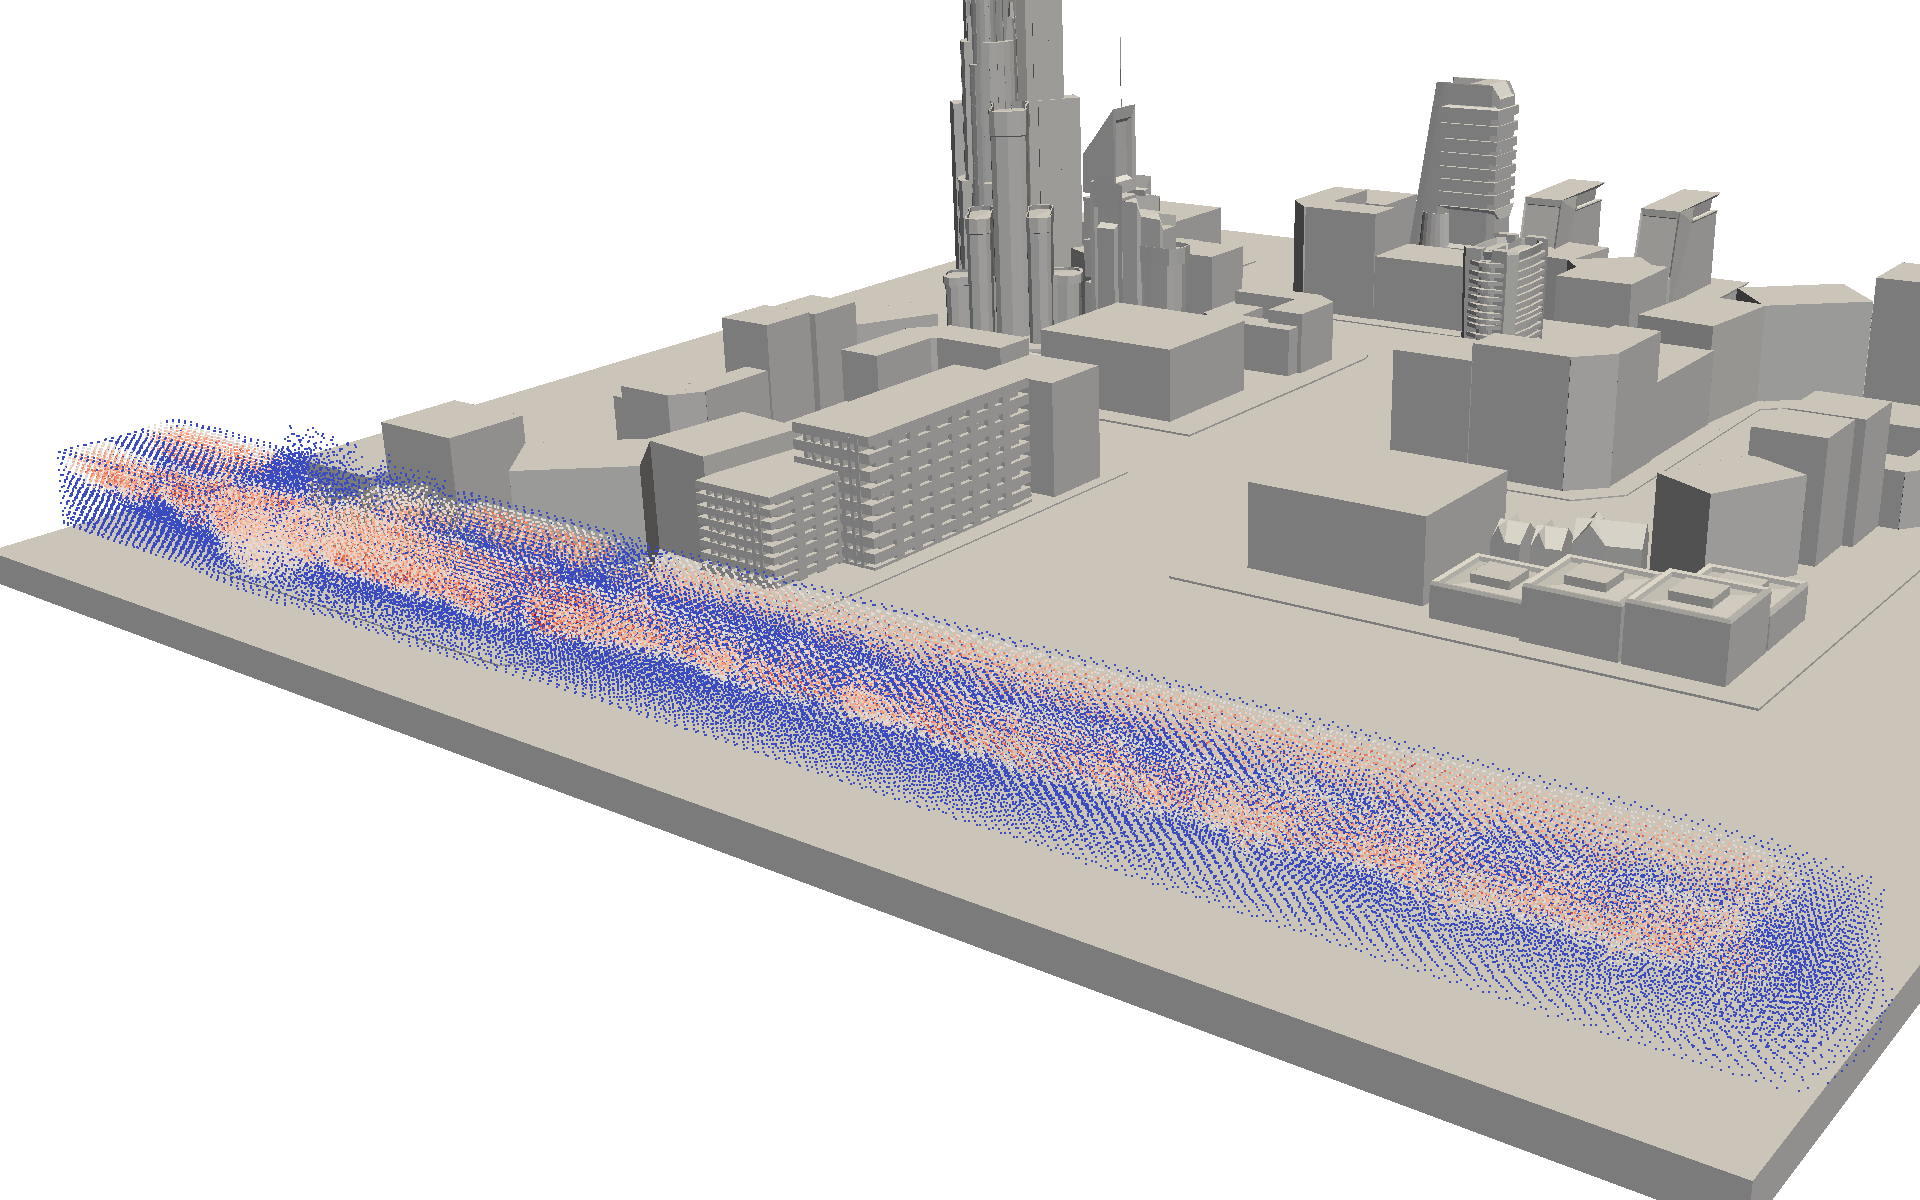
\includegraphics[width=.5\textwidth]{figures/press-2.png}
  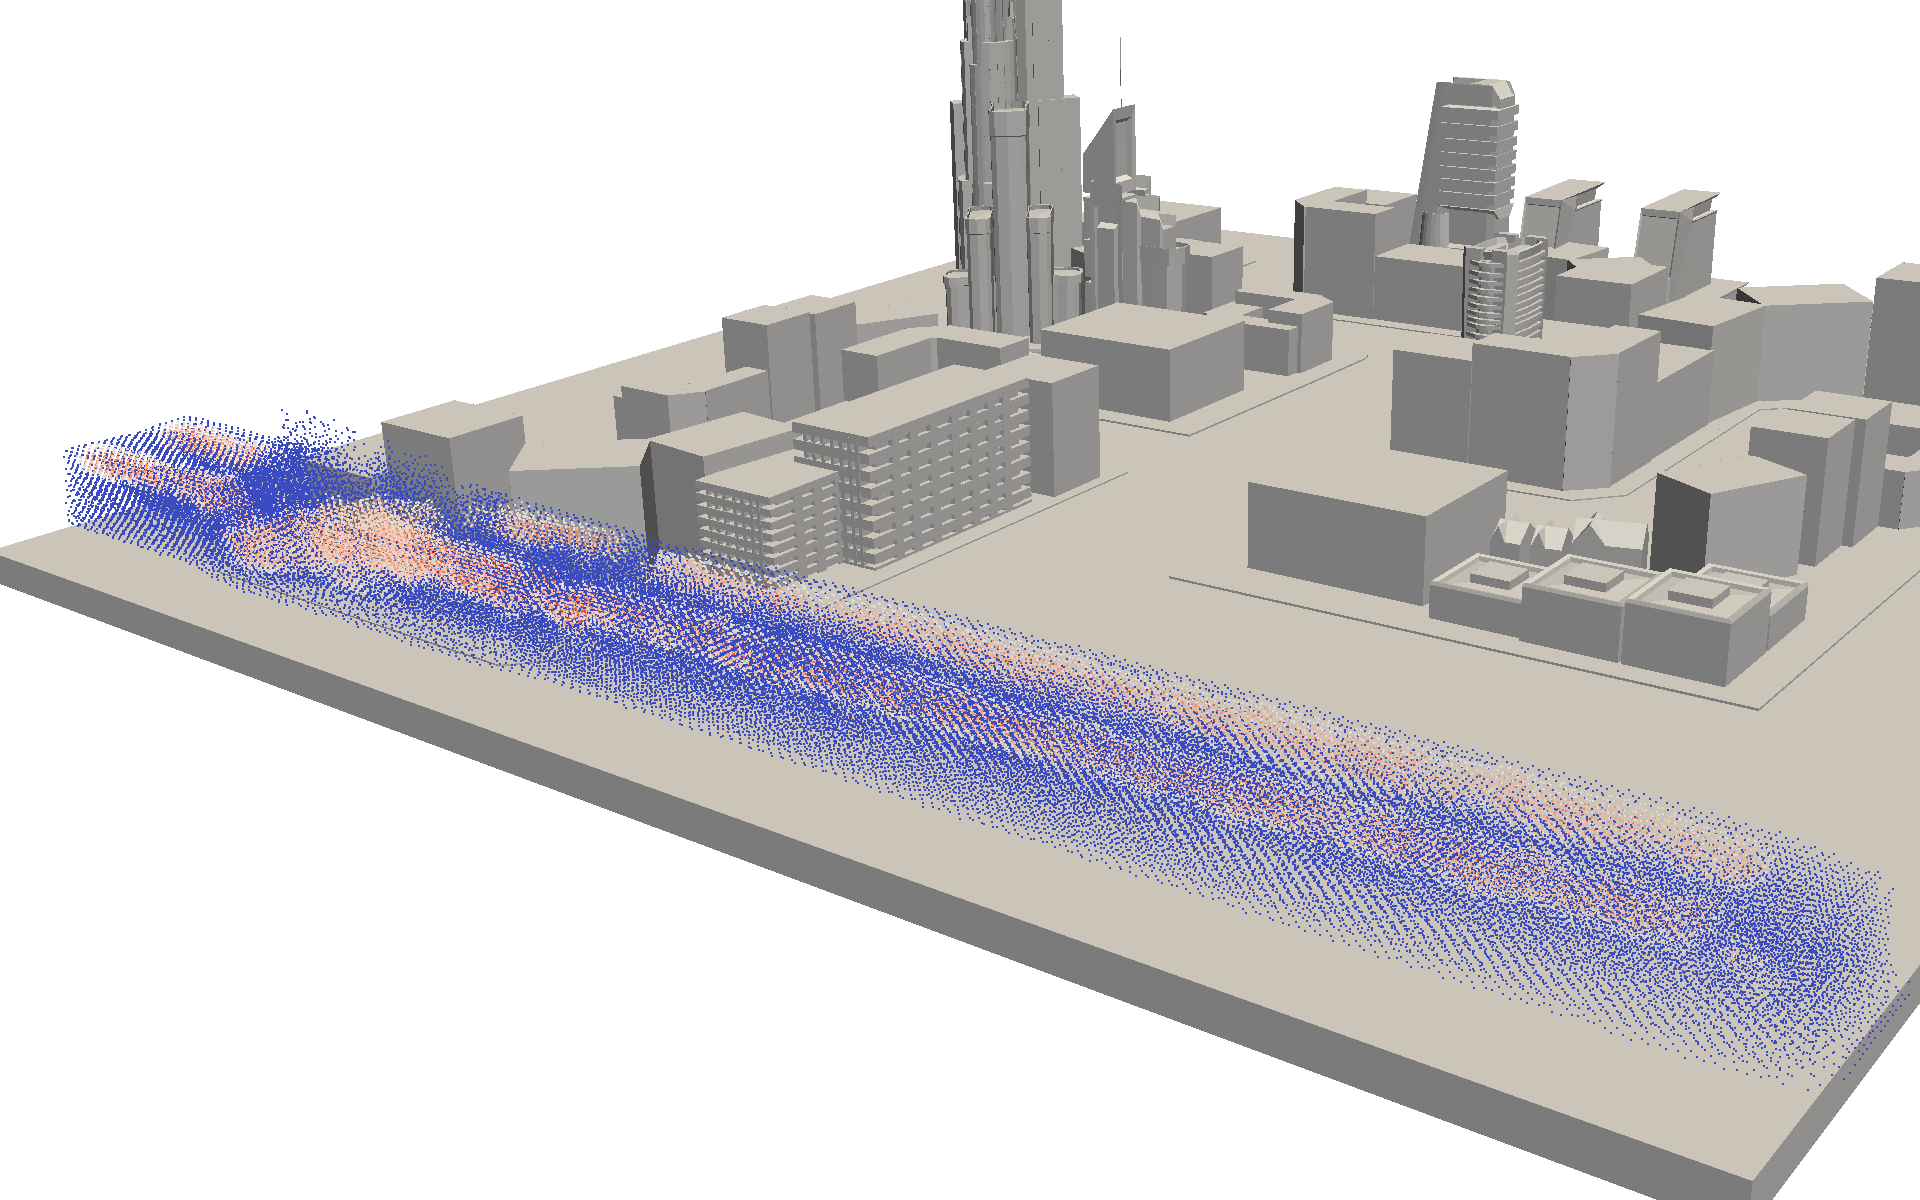
\includegraphics[width=.5\textwidth]{figures/press-3.png}
\end{frame}

%%%%%%%%%%%%%%%%%%%%%%%%%%%%%%%%%%%%%%%%%%%%%%%%%%%%%%%%%%%%%%%%%%%%%%%%%%%%%%%% 

\begin{frame}{Ιξώδες}
  \includegraphics[width=.5\textwidth]{figures/visc-0.png}
  \includegraphics[width=.5\textwidth]{figures/visc-1.png}\\
  \includegraphics[width=.5\textwidth]{figures/visc-2.png}
  \includegraphics[width=.5\textwidth]{figures/visc-3.png}
\end{frame}

%%%%%%%%%%%%%%%%%%%%%%%%%%%%%%%%%%%%%%%%%%%%%%%%%%%%%%%%%%%%%%%%%%%%%%%%%%%%%%%% 

\begin{frame}{Αριθμός γειτονικών σωματιδίων}
  \includegraphics[width=\textwidth]{figures/samples.png}
\end{frame}

%%%%%%%%%%%%%%%%%%%%%%%%%%%%%%%%%%%%%%%%%%%%%%%%%%%%%%%%%%%%%%%%%%%%%%%%%%%%%%%% 

\subsection{Ακτογραμμή}

\begin{frame}{Ώσεις}
  \includegraphics[width=.5\textwidth]{figures/impulses-0.png}
  \includegraphics[width=.5\textwidth]{figures/impulses-1.png}\\
  \includegraphics[width=.5\textwidth]{figures/impulses-2.png}
  \includegraphics[width=.5\textwidth]{figures/impulses-3.png}
\end{frame}

%%%%%%%%%%%%%%%%%%%%%%%%%%%%%%%%%%%%%%%%%%%%%%%%%%%%%%%%%%%%%%%%%%%%%%%%%%%%%%%%

\begin{frame}{\eng{Heatmap} ώσεων (1/3)}
  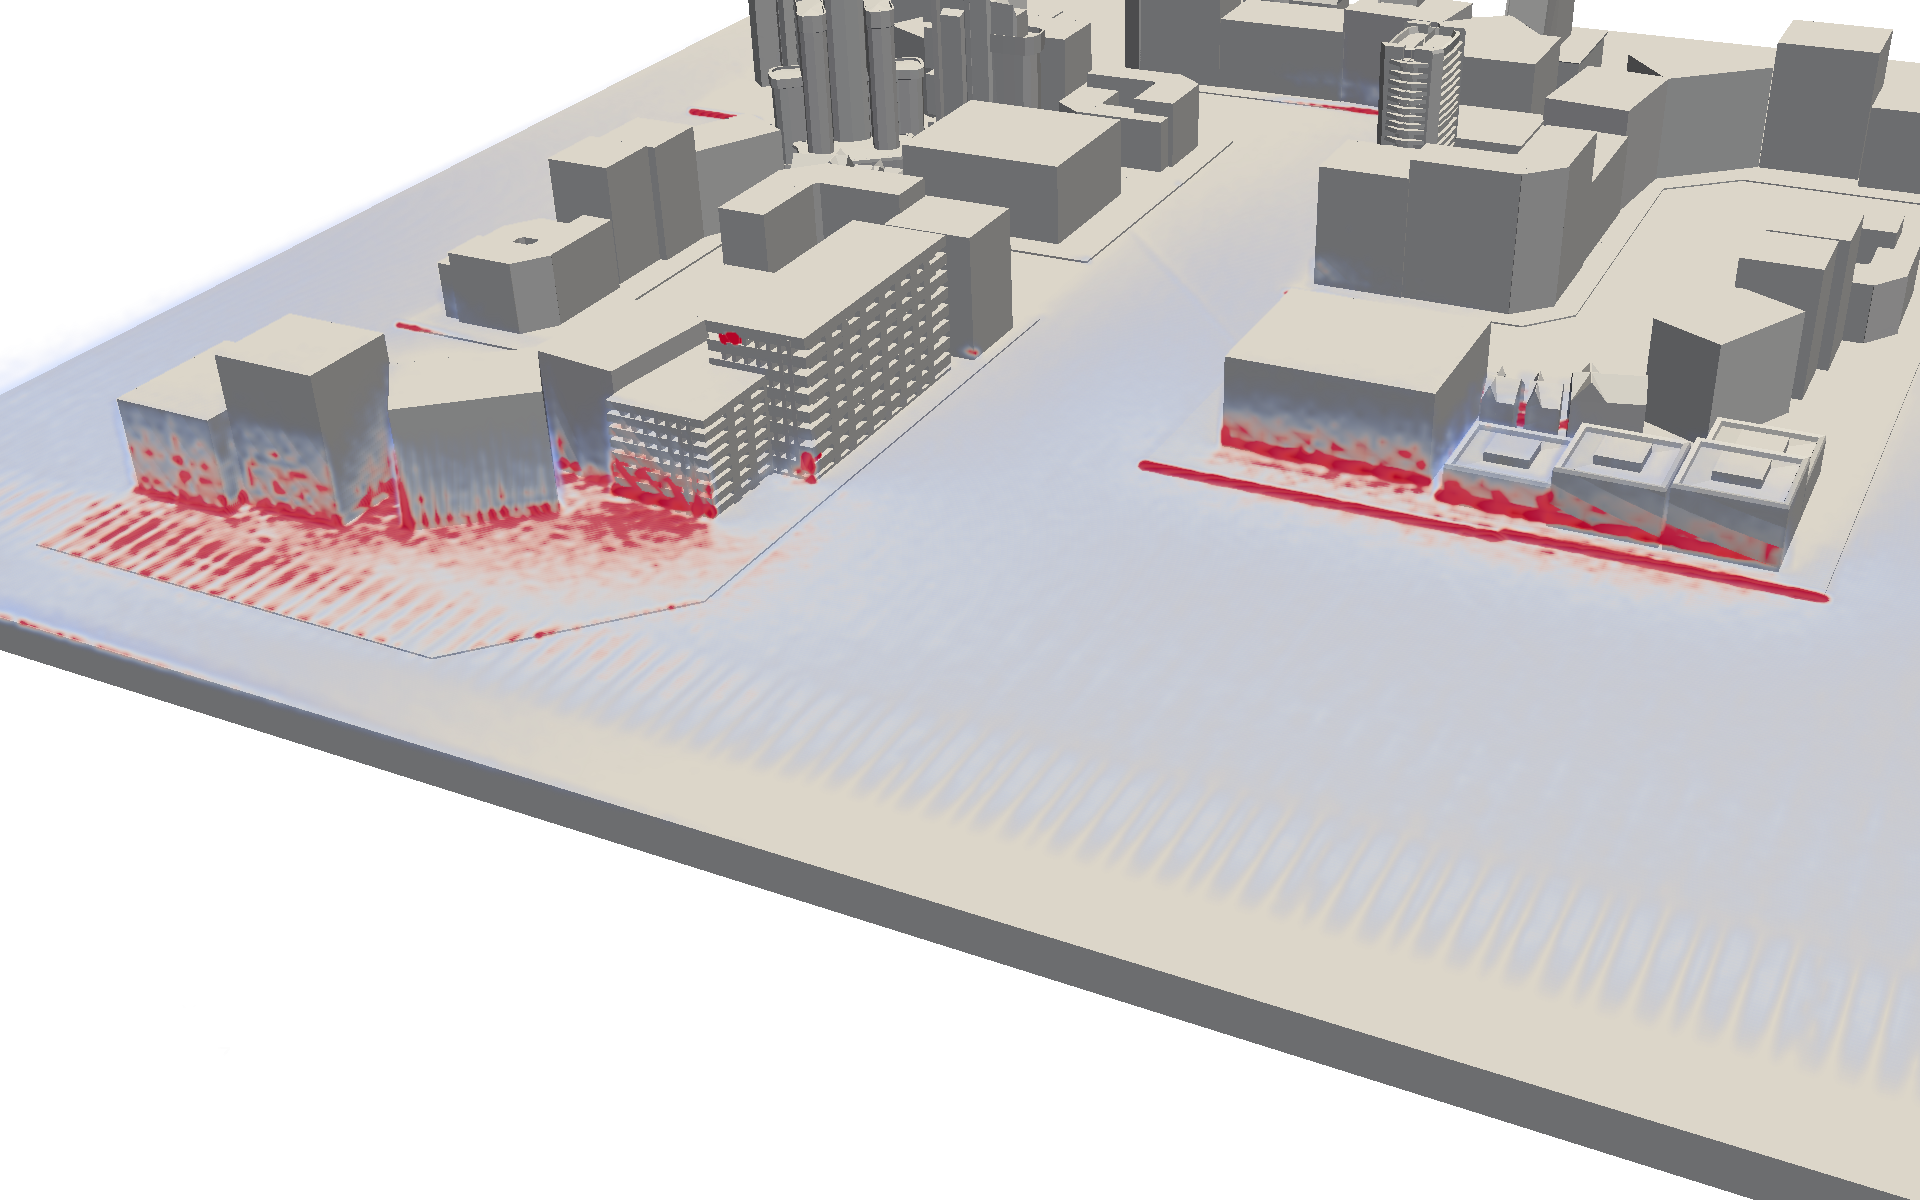
\includegraphics[width=\textwidth]{figures/impulse-heatmap-0.png}
\end{frame}

%%%%%%%%%%%%%%%%%%%%%%%%%%%%%%%%%%%%%%%%%%%%%%%%%%%%%%%%%%%%%%%%%%%%%%%%%%%%%%%%

\begin{frame}{\eng{Heatmap} ώσεων (2/3)}
  \includegraphics[width=\textwidth]{figures/impulse-heatmap-1.png}  
\end{frame}

%%%%%%%%%%%%%%%%%%%%%%%%%%%%%%%%%%%%%%%%%%%%%%%%%%%%%%%%%%%%%%%%%%%%%%%%%%%%%%%%

\begin{frame}{\eng{Heatmap} ώσεων (3/3)}
  \includegraphics[width=\textwidth]{figures/impulse-heatmap-2.png}
\end{frame}

%%%%%%%%%%%%%%%%%%%%%%%%%%%%%%%%%%%%%%%%%%%%%%%%%%%%%%%%%%%%%%%%%%%%%%%%%%%%%%%%

\begin{frame}{Αποτελεσματικότητα κυματοθραύστη}
  \includegraphics[width=\textwidth]{figures/if-city0-free.png}\\
  \includegraphics[width=\textwidth]{figures/if-city0-seawall.png}
\end{frame}


%%%%%%%%%%%%%%%%%%%%%%%%%%%%%%%%%%%%%%%%%%%%%%%%%%%%%%%%%%%%%%%%%%%%%%%%%%%%%%%% 

\section{}
\subsection{}
\begin{frame}
  \begin{center}
    \spacer\spacer\spacer\spacer\spacer\spacer
    Ευχαριστώ!\\
    \spacer\spacer\spacer\spacer\spacer\spacer
    Ερωτήσεις?
  \end{center}
\end{frame}

\end{document}

%%% Local Variables:
%%% mode: latex
%%% TeX-master: t
%%% End:
